%% The following is a directive for TeXShop to indicate the main file
%%!TEX root = diss.tex

\chapter{Background}
\label{ch:rw}

In this chapter, we provide the relevant background for this dissertation.
We begin by describing what haptics is with an overview of haptic technology and perception.
Next, we discuss the application space for haptics and why haptic experiences are increasingly important to design.
We then discuss the previous work in haptic experience design and \haxd tools, identifying why this is an area for improved understanding.
After, we discuss creativity support tools and design theory from non-haptic tools to provide inspiration and guiding principles.
Finally, we present the methodologies used in this dissertation.
Throughout the chapter, we contextualize this work and \haxd in both the haptics and HCI communities.


%%%%%%%%%%%%
%
% SECTION: What is haptics?
%
%%%%%%%%%%%%
\section{An Overview of Haptic Technology and Perception}
The term ``haptic" was coined by German researcher Max Dessoir \cite{Grunwald2008} to refer to the sense of touch, in a similar manner as ``optic" for vision and ``acoustic" for sound.
Today, it refers to both the study of the psychology and perception of the senses of touch, and frequently to technology that employs touch as a method of feedback.
Haptic technology is typically separated into two classes based on the main sense modality: \emph{tactile} sensations, perceived through the skin, and \emph{proprioception}, or the sense of body location and force.

\inlineHeading{Tactile Perception and Technology}
Tactile sensations rely on multiple sensory organs in the skin, each of which detect different properties, \eg, Merkel disks detect pressure or fine details, Meissner corpuscles detect fast, light sensations (flutter), Ruffini endings detect stretch, and Pacinian corpuscles detect vibration \cite{ChoiKuchenbecker2013}.
%Temperature and pain are also detected through \osC{todo}.
Of these, the Pacinian corpuscle is most targeted by technology through vibrotactile (VT) sensations, where vibrations stimulate the skin.
The most common example of this is smartphone vibrations.
VT actuators can take may forms. Eccentric mass motors (sometimes ``rumble motors" or, when small, ``pager motors") are found in many mobile devices and game controllers, and are affordable but inexpressive.
%An unbalanced mass is mounted on the motor, which provides dramatic shaking of the device.
More expressive are tactors, or voice coils, implemented in a variety of ways and offering two degrees of freedom: frequency and amplitude.
Piezo actuation is a very responsive technique that is typically more expensive.
% One of the more common and expressive is the C2 tactor, intended to directly stimulate the skin through contact or a thin membrane; the tactile animation project [] uses an array of C2 tactors.
While tactors directly stimulate the skin, linear resonant actuators (LRAs) shake a mass back and forth to vibrate a handset in an expressive way; a common research example is the Haptuator \cite{Yao2010}.
Instead of directly stimulating the skin, this actuator typically shakes another device held by the user, such as a mobile device \cite{Yoo2014} or pen \cite{Culbertson2014}.
As of writing (2016), this type of actuator is increasingly deployed in mobile contexts (\eg, the Apple Watch Taptic engine).


\inlineHeading{Proprioception and Force Feedback}
Proprioception, the sense of force and position, is synthesized from multiple sensors as well: the muscle spindle (embedded in muscles), golgi-tendon organ (GTO) in tendons, and tactile and visual cues \cite{Kandel2000}.
Common devices include Geomagic Touch (previously the Sensable PHANTOM) and Falcon devices, offering three degrees-of-freedom: force in three directions and torque in three orientations.
At other times, entire screens might push back on the user in a single degree-of-freedom.


\inlineHeading{Multimodal interaction}
Similar to vision and audio, haptic perception is susceptible to illusions \cite{Hayward2016,Hayward2008}.


%%%%%%%%%%%%
%
% SECTION: Why should we care about haptics?
%
%%%%%%%%%%%%
\section{The Value of Haptic Experiences}


\subsection{Education}
Haptic technology has the potential to improve educational resources, especially to those lacking resources.
Montessori methods have long espoused the value of physical learning aids, especially using physical \emph{manipulatives} \cite{Montessori1917}.
There is evidence to support these techniques: in a meta-analysis of 55 studies, \citet{Carbonneau2013} found that physical manipulations improve several learning outcomes, with influence by other instructional variables.
Studies of gestures have also found value in students ``being the graph" by physically acting out mathematical shapes, grounding abstract knowledge in embodied experience \cite{Gerofsky2010}.
These techniques have roots in constructivist learning, where learners use existing understandings as a \emph{transitionary object} to understand new concepts \cite{Papert1980}.

Haptic technology is well-positioned to support embodied learning, and there is early evidence for its efficacy.
Haptic feedback has been shown to improve temporal aspects when training motor skills \cite{Feygin2002}.
In a study for molecular chemistry education, \citet{Sato2008} found students had higher test scores when they interacted with their haptic learning interface; students reported engagement.
In \autoref{ch:applications} we describe results from an early learning interface for low-cost haptic displays \cite{Martinez2016}, showing that haptic technology can improve engagement and make lasting impressions.



\subsection{Immersive Media}
A popular application for haptic experiences is augmented, immersive media experiences.
Actuated tactile feedback has been used as early as 1959 in the movie \emph{The Tingler}  \cite{IJsselsteijn2003}.
4D theatres and theme park rides use bursts of air or water sprays to engage the audience.
Companies like D-Box (\url{www.d-box.com}) augment films with haptic tracks that both low-frequency movements and high-frequency vibrations, and can be found in theatres across the world.
Buttkicker (\url{www.thebuttkicker.com}) also augments 4D theatres, and provides products for home theatre setups.

Haptic experiences are also increasingly of interest in virtual reality (VR) environments.
Skin stretch techniques, explored in \cite{Guinan2014} and now commercialized by Tactilcal Haptics (\url{tacticalhaptics.com}), augments virtual-reality setups by simulating forces and torques using handheld controllers, lending stronger immersion for virtual environments and VR games.
Haptic Turk \cite{Cheng2014} and TurkDeck \cite{Cheng2015} are innovative explorations of high-fidelity haptic experiences in virtual environments using people as actuators.
Impacto uses electrical muscle stimulation and a solenoid actuator to create wearable haptic feedback with both kinaesthetic and tactile feedback \cite{Lopes2015}.


Previous work has also attempted to add greater immersion to broadcast media by including haptic sensations.
\citet{Modhrain2001} present an early vision of Touch TV, using active touch with two-DOF actuators embedded in remote controllers.
\citet{Gunther2002} studied a full-body vibrotactile suit to create music-like ``cutaneous grooves", helping to identify the artistic space of VT sensations, including concerts with tactile compositions.
More recently, the proliferation of online streaming video has developed opportunities to add haptic sensations using novel data structures.
Tactile Movies \cite{Kim2009} looks into augmenting movies with spatial VT feedback, including an authoring interface.
The Haptic Application Meta Language (HAML)\cite{Eid2006} is an XML-based data format for adding haptics to MPEG-7 video, eventually augmented with the HAML Authoring Tool (HAMLAT) \cite{,Ferre2008}.
\citet{AbdurRahman2010} eventually adapted an XML approach to YouTube, and \citet{Gao2013} developed related online MPEG-V haptic editing.

Augmented media experiences, or haptic-audiovisual (HAV) content \cite{Danieau2013},  have used different methods of input.
One approach is to use camera motion sourced from accelerometers \cite{Danieau2012} to actuate audience members' hands and head in a HapSeat \cite{Danieau2013a,Danieau2012a}.
Later editable with H-Studio \cite{Danieau2013c}, this work has proposed the concept of Haptic Cinemotography \cite{Danieau2014}, including basic principles of composition when combined with video \cite{Guillotel2016}.
Other approaches include automatic conversion of audio content
Several studies have looked into automatic conversion from audio streams \cite{Lee2013,Chang2005,Hwang2014} or video streams \cite{Kim2014} to VT or force-feedback output.

\subsection{Healthcare}

Therapy, Social, affective, guidance, accessibility, medical, mobile and ubiquitous, calm computing, ...



%%%%%%%%%%%%
%
% SECTION: Why should we care about haptic experience design tools? What is the precise problem this dissertation is solving?
%
%%%%%%%%%%%%
\section{Previous Efforts for Haptic Experience Design}
\osC{Should we do a separate section for Creativity and Design itself? Or is that a subsection?}



%%%%%%%%%%%%
%
% SECTION: What other inspirations can we draw from? How are we approaching the above-mentioned problem? What scope is reasonable.
%
%%%%%%%%%%%%
\section{Non-Haptic Design and Creativity Tools}






%%%%%%%%%%%%
%
% SECTION: Methodology. How will we transform the above-mentioned approach into knowledge? How can we study our solutions?
%
%%%%%%%%%%%%
\section{Methodology}







%%%%%%%%%%%%%%%
%%%%
%%%% SECTION: Haptics
%%%%
%%%%%%%%%%%%%%%
%%%\section{Haptics}
%%%The word ``haptics" stems from the Greek word ``haptos", meaning to grasp or feel \osC{cite, confirm}.
%%%Today, we typically use it to refer to both technology and perception involving the senses of touch.
%%%
%%%Haptic technology is typically separated into two classes based on the main sense modality: \emph{tactile} sensations, perceived through the skin, and \emph{proprioception}, or the sense of body location and force. 
%%%We begin with a brief overview of the perception of touch, then discuss types of haptic technology, and conclude with major application areas for haptics.
%%%
%%%\subsection{Perception}
%%%
%%%
%%%Proprioception, on the other hand, is synthesized from the muscle spindle and golgi-tendon organ (GTO), as well as tactile and visual cues \cite{Kandel2000}.
%%%Common devices include Geomagic Touch (previously the Sensable PHANTOM) and Falcon devices, offering three degrees-of-freedom: force in three directions and torque in three orientations.
%%%Simpler one degree-of-freedom devices are used in education, prototyping, and experimentation.
%%% Devices include the Twiddler (a haptic knob from UBC) and the HapKit (a low-cost paddle by the Stanford CHARM lab).
%%% %the latter is used in the CyberHap side project.
%%%
%%%
%%%Multiple senses
%%%
%%%Illusions
%%%
%%%\subsection{Technology}
%%%
%%%The most common consumer-facing tactile technology is vibrotactile (VT), where vibrations stimulate the skin.
%%%Eccentric mass motors (sometimes ``rumble motors" or, when small, ``pager motors") are found in many mobile devices and game controllers.
%%%%An unbalanced mass is mounted on the motor, which provides dramatic shaking of the device.
%%%However, these have only a single degree of freedom: the input voltage or current, which corresponds to the combined amplitude and frequency of the device.
%%%Eccentric mass motors are cheap, salient, widespread, but inexpressive.
%%%
%%%More expressive are tactors, or voice coils, implemented in a variety of ways.
%%%Behaving similar to small speakers, tactors offer two degrees of freedom: frequency and amplitude, and are typically more responsive than rumble motors.
%%%One of the more common and expressive is the C2 tactor, intended to directly stimulate the skin through contact or a thin membrane; the tactile animation project (\autoref{ch:hapticanimation}) uses an array of C2 tactors.
%%%Another common device, commonly used in research or prototyping, is the Haptuator \cite{Yao2010}.
%%%Instead of directly stimulating the skin, this actuator typically shakes another device held by the user, such as a mobile device \cite{Yoo2014}, pen \cite{Culbertson2014}, or other handle.
%%%Both the haptic instrument (\autoref{ch:hapticinstrument}) and Macaron editor (\autoref{ch:hapticexamples}) use Haptuators.
%%%
%%%\subsection{Applications}
%%%
%%%%VT devices can be used alone or put together into grids.
%%%%Sensory illusions in touch, such as phantom tactile sensations \cite{Alles1970}, create illusory vibrations in between two or more VT actuators.
%%%%Seo and Choi created a perceived motion flow between two vibrators mounted on the ends of a handheld device by controlling their intensity  \cite{Seo2010}.
%%%%Lee and colleagues created across-the-body and out-of-the-body illusions on a mobile device using up to four % inexpensive 
%%%%linear resonant actuators \cite{Lee2012a}.
%%%%The Tactile Brush algorithm \cite{Israr2011a} combined phantom tactile sensations and apparent tactile motion to render high-resolution and moving haptic patterns on the back using a coarse grid of VT actuators. 
%%%%Other spatio-temporal VT illusions such as the  ``cutaneous rabbit"  \cite{Tan2009} and Tau and Kappa effects \cite{Hayward2008} can also be used with VT arrays.
%%%
%%%
%%%
%%%%\subsection{Applications}
%%%%An early cinematic use of haptic feedback was in a multisensory experience called \emph{Percepto} used for the movie ``The Tingler" in 1959 \cite{IJsselsteijn2003}. %
%%%%%G. Riva, F. Davide, and W.A. IJsselsteijn, �Presence in the Past: What Can We Learn from Media History?,� Being There: Concept, Effects and Measurements of User Presence in Synthetic Environments, IOS Press, 2003, Amsterdam, The Netherlands, pp. 17-40.
%%%%Theater seats were equipped with vibrating devices that buzzed the audience during events in the movie.
%%%%Current 4D theaters, rides, shows, and gaming arcades are equipped with sophisticated motion platforms (e.g. D-Box, http://www.d-box.com) that supplement visual scenes with subtle and synchronized movements.
%%%%Large tactile transducers (such as Buttkickers, www.thebuttkicker.com) are also common with gaming and music content that shake the entire seat using the sound stream, therefore allowing users to feel `bumps' during musical beats and gameplay.   
%%%%Custom editors (such as D-Box Motion Code Editor) and software plugins are provided to media designers that overlaid the visual and audio content with haptics, and allow designers to generate, tune and save frame-by-frame haptic content in an allocated track for it to play simultaneously with the media content. 
%%%
%%%%In contrast to displacing the entire user body, recent multichannel haptic devices create percepts of dynamic and localized haptic sensations directly on the user's skin \cite{Israr2011} and in the mid-air \cite{Wilson2014}.
%%%%%  Designers (and researchers) for these technologies must have 
%%%%Use of these technologies requires
%%%%extensive programming experience, knowledge of hardware and background in haptic sciences to generate expressive and meaningful haptic content. 
%%%%% Due to the lack of
%%%%Without guiding principles or haptic libraries,  content generation schemes are complex, device-specific and time consuming. 
%%%%Recently, Schneider and colleagues introduced  the tool ``FeelCraft" for end users to create expressive haptic content using a library of \emph{feel effects} \cite{SchneiderAsiaHaptics2014}.
%%%%By tuning parameters of these effects, users could personalize  haptic content, embed it in games and share effects with other users.
%%%%Similar devices and authoring schemes are also developed for online social interactions using custom multi-actuator haptic devices \cite{Kim2009,Tsetserukou2009,Paneels2013}.%Tsetserukou, D. and Neviarouskaya, A. iFeel_IM!: augmenting emotions during online communication. Comp. Graphics & Applications 30 (2009), IEEE, 72-80.
%%%%
%%%
%%%
%%%
%%%
%%%
%%%%%%%%%%%%%%%
%%%%
%%%% SECTION: Haptic Design Tools
%%%%
%%%%%%%%%%%%%%%
%%%\section{Haptic Design Tools}
%%%Currently, haptic designers have access to a limited number of hardware and software platforms, a set of philosophical design perspectives, and authoring tools.
%%%
%%%\subsection{Platforms}
%%%Many software libraries aim to support developers.
%%%The UPenn Texture Toolkit contains 100 texture models created from recorded data, rendered through VT actuators and impedance-type force feedback devices \cite{Culbertson2014}.
%%%The HapticTouch Toolkit \cite{Ledo2012} and Feel Effect library \cite{Israr2014} control sensations using semantic parameters, like ``softness" or ``heartbeat intensity" respectively.
%%%%and Feel Effects  provide examples for vibrotactile actuators, like those found in game controllers and mobile devices.
%%%Vibrotactile libraries like Immersion's Haptic SDK (immersion.com) connect to mobile applications, augmenting Android's native vibration library.
%%%%FeelCraft's plugin architecture connects feel effects to various media types \cite{SchneiderAsiaHaptics2014}.
%%%Force feedback devices have software platforms like CHAI3D (chai3d.org), H3D (h3dapi.org), and OpenHaptics (geomagic.com). 
%%%
%%%Hardware prototyping platforms like
%%%Arduino (arduino.cc) provide an open source microcontroller % platform 
%%%and development platform % environment
%%%for physical prototyping.
%%%Phidgets (phidgets.com) facilitate rapid hardware prototyping with over 20 programming languages 
%%%\cite{Greenberg2001}.
%%%More recently, Wooden Haptics gives open-source access to fast laser cutting techniques for force feedback development \cite{Forsslund2015}, and
%%%% Projects like 
%%%faBrickation streamlines prototyping for 3D printing \cite{Mueller2014}. % and other manufacturing techniques.
%%%These platforms, especially Arduino, have made significant improvements to enable rapid iteration and hardware sketching.
%%%However, I believe we can do much better: these platforms require programming, hardware, and haptics expertise, and include inherent time costs like compilation, uploading, and debugging.
%%%
%%%\subsection{Design Perspectives}
%%%Some higher-level perspectives offer outcome targets or design attitudes to guide haptic practitioners.
%%%``DIY Haptics'' categorize  feedback styles and design principles \cite{Hayward2007,MacLean2008}.
%%%``Ambience'' is proposed as one target for a haptic experience \cite{MacLean2009}.
%%%Haptic illusions can serve as concise ways to explore the sense of touch, explain concepts to novices and inspire interfaces \cite{Hayward2008}.
%%%``Simple Haptics'', epitomized by \emph{haptic sketching}, emphasizes rapid, hands-on exploration of a creative space \cite{Moussette2010,Moussette2011}. % with a design perspective \cite{Moussette2010,Moussette2011}.
%%%Haptic Cinematography \cite{Danieau2014} uses a film-making lens, discussing physical effects using cinematographic concepts.
%%%The notion of distributed cognition \cite{Hutchins1995} has particular relevance for haptic design, % provides an important perspective for haptic design in particular, 
%%%suggesting that people situate their thinking both in their bodies and in the environment.
%%%Haptics courses are taught with a variety of foci including perception, control, and design, providing students with an initial repertoire of skills \cite{Okamura2012, Jones2014}.
%%%
%%%Haptics has often made use of metaphors from other fields.
%%%Haptic icons  \cite{MacLean2003}, tactons \cite{Brewster2004}, and haptic phonemes \cite{Enriquez2006} are small, compositional, iconic representations of haptic ideas.
%%%Touch TV \cite{Modhrain2001},  tactile movies \cite{Kim2009}, haptic broadcasting \cite{Cha2009}, and Feel Effects \cite{Israr2014} attempt to add haptics to existing media types, especially video.
%%%
%%%Musical analogies have frequently been used to inspire haptic design tools, especially VT sensations. %unique.
%%%The Vibrotactile Score, a graphical editing tool representing vibration patterns as musical notes, is a major example \cite{Lee2012, Lee2009}.
%%%%The vibrotactile score provides an abstraction beyond low-level parameters and can draw from a musician's familiarity with the notation.
%%%Other musical metaphors include the use of rhythm, often represented by musical notes and rests \cite{Ternes2008,Brown2005,Chan2008, Brown2006a}.
%%%Earcons and tactons are represented with musical notes \cite{Brewster1993,Brewster2004}, complete with
%%%tactile analogues of crescendos and sforzandos \cite{Brown2006}.
%%%The concept of a VT concert found relevant tactile analogues to musical pitch, rhythm, and timbre for artistic purposes \cite{Gunther2002}.
%%%Correspondingly, tactile dimensions have been also been used to describe musical ideas \cite{Eitan2010}.
%%%
%%%
%%%%\subsection{Language of Tactile Stimuli}
%%%The language of tactile perception, especially affective (emotional) terms, is another way of framing haptic design.
%%%%The language of tactile stimuli has a long history in psychological studies \cite{Okamoto2013}.
%%%Many psychophysical studies have been conducted to determine the main tactile dimensions with both synthetic haptics and real-world materials  \cite{Enriquez2003,Okamoto2013}.
%%%Language is a promising way of capturing user experience \cite{Obrist2013}, and can reveal useful parameters, e.g., how pressure influences affect \cite{Zheng2012}.
%%%Tools for customization by end-users, rather than expert designers, are another way to understand perceptual dimensions \cite{Seifi2014, Seifi2015}.
%%%However, this work is far from complete; touch is difficult to describe, and some even question the existence of a tactile language \cite{Jansson-Boyd2011}.
%%%%There is a clear need to empirically investigate the subjective experience of touch-based interfaces, for which phenomenology is ideal \cite{Creswell2013, Moustakas1994}.
%%%%Start with hapticons, tactons, vibrotactile icons, Earcons, Auditory icons...
%%%%Participants described two different sensations, one oscillating at 16 Hz and the other at 250 Hz.
%%%
%%%
%%%
%%%
%%%	% Guest, S., Dessirier, J., Mehrabyan, A., McGlone, F., Essick, G., Gescheider, G., Fontana, A., Xiong, R., Ackerley, R., and Blot, K., “The Development and Validation of Sensory and Emotional Scales of Touch Perception,” Attention, Perception, & Psychophysics, vol. 73:2, pp. 531-550, 2011.
%%%%
%%%
%%%
%%%
%%%
%%%\subsection{Authoring Interfaces}
%%%As long as designers have considered haptic effects for entertainment media, they have needed compositional tools % to facilitate their design 
%%%\cite{Gunther2002}.
%%%A great deal of previous work has focused on how to prototype or author haptic phenomena using non-programming methods. 
%%%
%%%Many user-friendly interfaces help designers create % control 
%%%haptic sensations, especially with vibrotactile devices.
%%%The Hapticon editor \cite{Enriquez2003}, Haptic Icon Prototyper \cite{Swindells2006}, and posVibEditor \cite{Ryu2008} use graphical mathematical representations to edit either waveforms or profiles of dynamic parameters (torque, frequency) over time.
%%%The Vibrotactile Score \cite{Lee2009} was shown to be generally preferable to programming in C and XML, but required familiarity with musical notation \cite{Lee2012}. 
%%%%Mobile tools make haptic design more accessible.
%%%The Demonstration-Based Editor \cite{Hong2013} allows control of frequency and intensity by moving graphical objects on a touchscreen.
%%%%mHIVE, a Haptic Instrument \cite{Schneider2014} controls frequency, intensity, waveform and amplitude envelope of two tactors with touchscreen gestures.
%%%Similar to the SPIN lab's Haptic Instrument (mHIVE, \autoref{ch:hapticinstrument}), this mobile tool was shown to be intuitive and easy to use for exploration or communication, but faltered when refining more elaborate sensations. %for a set context.
%%%
%%%Commercially, Apple's end-user vibration editor has been present in iOS since 2011 (iOS 5) but only produces binary on/off timing information.
%%%Immersion provides two tools: TouchSense Engage is a software solution for developers, while Touch Effects Studio lets users enhance a video from a  library of tactile icons supplied on a mobile platform.
%%%Vivitouch Studio allows for haptic prototyping of different effects alongside video (screen captures from video games) and audio, and supports features like A/B testing \cite{Swindells2014}.
%%%%More recently, Vivitouch Studio \cite{Swindells2014} allows for haptic prototyping of different effects alongside video (screen captures from video games) and audio, including features like A/B testing for simultaneous comparison of haptic content and exporting of a haptic video channel.
%%%
%%%
%%%The control of multi-actuator outputs has been explored by TactiPEd \cite{Paneels2013}, Cuartielles' proposed editor \cite{Cuartielles2012}, and the tactile movie editor \cite{Kim2009}; the latter combined spatial and temporal control using a tactile video metaphor for dense, regular arrays of tactile pixels (``taxels"), including a feature of sketching a path on video frames. 
%%%However, these approaches embrace the separate control of different actuators, rather than a single perceived sensation produced by the multi-actuator device, which we address with tactile illusions in \autoref{ch:hapticanimation}.
%%%
%%%%The hapticon editor \cite{Enriquez2003}, haptic icon prototyper \cite{Swindells2006}, posVibEditor \cite{Ryu2008}, and Immersion's Haptic Studio (www.immersion.com) use a graphical representation to edit either waveforms or profiles of dynamic parameters (such as, torque) over time.
%%%
%%%%Both emphasize exploration and broad manipulation rather than finely controlled end results.
%%%
%%%
%%%
%%%
%%%%%%%%%%%%%%%
%%%%
%%%% SECTION: Design
%%%%
%%%%%%%%%%%%%%%
%%%\section{Non-Haptic Design Theory}
%%%In this section, we present related work on non-haptic design organized into three major elements: problem preparation, hands-on design, and collaboration.
%%%
%%%\subsection{Problem Preparation}
%%%Creative tasks, like design, are often defined as the recombination of existing ideas, with a twist of novelty or spark of innovation by the individual creator \cite{Warr2005}.
%%%Also known as the ``problem setting" \cite{Schon1982}, ``analysis of problem" \cite{Warr2005}, or ``collect" \cite{Shneiderman2000} step, problem preparation involves getting a handle on the problem,  drawing inspiration from previous work. %, and and establishing a first general approach with which to attempt a solution.
%%%Sch\"{o}n demonstrated that designers initially frame their problems before developing a solution \cite{Schon1982}.
%%%Sch\"{o}n also describes the designer's repertoire, their collected experience, which aids in design.
%%%External examples are especially useful for inspiration and aiding initial design \cite{Herring2009,Buxton2007}, which we explore in \autoref{ch:hapticexamples}.
%%%
%%%
%%%%%Framing, finding the appropriate metaphor for thinking about the problem \cite{Schon1982}.
%%%%When encountering a new problem, a designer begins \emph{framing}, finding the appropriate metaphor for thinking about the problem, typically drawn from her experience.
%%%%In this way, metaphors that people already understand can be used to learn about new situations as a transitionary object \cite{Papert1980}.
%%%%%Framing involves transforming the problem so that the designer can get a handle on it and begin to make progress.
%%%%\emph{Framing} could involve a set of constraints upon the design problem, a list of requirements, or notational language to describe the problem.
%%%%The more we can say about the problem, the more we can make progress on the solution.
%%%%
%%%%When \emph{framing}, designers draw from a \emph{repertoire} of their own previous experience that guides their design, storing cases, images, understandings, and actions \cite{Schon1982}.
%%%%This approach is widespread in the haptics literature (e.g., ``haptic icons"  \cite{MacLean2003}, ``touch TV" \cite{Modhrain2001}), suggesting that we often have to rely on outside metaphors to describe concepts in haptics.
%%%%
%%%%Designers draw both from their \emph{repertoire} and from others' design \emph{examples}.
%%%%While other sources sometimes use ``example" to refer to previously-encountered case studies \cite{Schon1982}, we consider those as part of the \emph{repertoire} and use ``example" exclusively to refer to externalized resources.
%%%%In other fields of design, designers clip, store, and display \emph{examples} for inspiration \cite{Buxton2007} (\autoref{fig:corkboard}).
%%%%Industrial designers collect various knobs and materials, and web designers bookmark sites \cite{Herring2009}.
%%%%Managing these \emph{examples} effectively is already a significant task even in these more visual fields.
%%%%%; with haptics, which often involves both software and hardware, this becomes a serious barrier.
%%%%To work effectively with \emph{examples}, we need to have ways to capture, visualize, and recall them \cite{Herring2009}.
%%%
%%%\subsection{Hands-On Design}
%%%There has recently been a shift in how we interpret the act of thinking.
%%%No longer is thinking relegated to the head; cognition is now seen as being situated in the physical world \cite{Hutchins1995}.
%%%The designer must iteratively generate a varied set of initial ideas  (ideation) and then prune them (evaluation), repeating this step many times to settle on a single design \cite{Buxton2007}.
%%%Working with multiple ideas simultaneously is a boon to good design.
%%%Developing interfaces in parallel can facilitate generation and evaluation, delaying commitment to a single design \cite{Hartmann2008, Resnick2008}, while
%%%in groups, sharing multiple designs improves variety and quality of designs \cite{Dow2011}.
%%%
%%%
%%%Sketching supports ideation, evaluation, and multiple ideas,
%%%allowing the designer to
%%%explicitly make moves in a game-like conversation with the problem \cite{Schon1982}.
%%%It is so important that some researchers declare it to be the fundamental language of design, like mathematics is the language for scientific thinking \cite{Cross2006}.
%%%The power of sketching, according to Cross, is contained in its ability to describe a partial model of a proposed design or problem.
%%%Detail can be subordinated, allowing a designer to zoom-in, solve a problem, and then
%%%abstract it away when returning to a high-level view.
%%%%\osC{cut this paragraph - should some of it be incorporated?}
%%%This has implications for software tools: designers must easily navigate the design space with undo, copy and paste, and a history of progress, creating tools with a ``high ceiling" and ``wide walls" \cite{Resnick2008}.
%%%
%%%
%%%\subsection{Collaboration}
%%%Design is a collaborative process with the potential for generating more varied ideas \cite{Warr2005}, and is important for creativity support tools \cite{Resnick2008,Shneiderman2000}.
%%%Although sometimes group dynamics influence the design process negatively, proper group management and sharing of multiple ideas results in more creativity and better designs \cite{Herring2009}.
%%%Shneiderman in particular has championed collaboration in design \cite{Shneiderman2000}, and suggests two different types of collaboration to be supported by creativity tools: \emph{relating}, informal discussions with colleagues, and \emph{donating}, disseminating information to the public/annals of time.
%%%Orthogonal to these intended purposes (relating and donating) is the collaboration context.
%%%Computer-supported collaborative work often separates interactions into four contexts ordered into two dimensions: collocated (same location) or distributed (different locations), and synchronous (simultaneous)  or asynchronous (at different times) \cite{Ellis1991}.
%%%Collaboration is notable because it is inherently challenging to haptic design: two people can look at the same image or hear the same sound from across a room, but touch is a local sense, far easier in a collocated, synchronous setting.
%%%We explore collaboration with the Haptic Instrument (\autoref{ch:hapticinstrument}) and the FeelCraft and HapTurk side-projects (described in \autoref{ch:haxd}).
%%%
%%%
%%%% (\autoref{tab:groupware}).
%%%%Considering these different contexts illuminates specific goals when supporting haptic experience design.
%%%
%%%%\begin{figure}[tbp] %  figure placement: here, top, bottom, or page
%%%%   \centering
%%%%   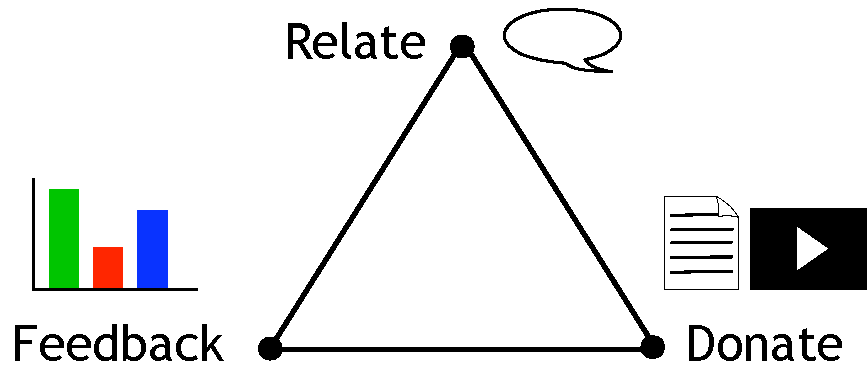
\includegraphics[width=0.33\textwidth]{figures/CollaborateSubProcesses2} 
%%%%   \caption{Collaboration sub-activities. Designers work collaboratively in a continuum between \emph{donating}, \emph{relating}, and gathering \emph{feedback}.}
%%%%   \label{fig:collaborate:sub:activities}
%%%%\end{figure}
%%%
%%%%\subsection{Challenge - Distributed Haptics}
%%%
%%%%However, collaboration in the remote or asynchronous case is more challenging.
%%%%Haptics has long been examined in remote collaboration both with force feedback \cite{Kim2004} and tactile \cite{Chan2008} mechanisms.
%%%%Remote collaboration to support haptics, on the other hand, is a different beast.
%%%
%%%%\subsubsection{Asynchronous collaboration}
%%%%Collocated collaboration is common and well supported in haptics.
%%%%In the synchronous case, \emph{relating} is a common activity, e.g., getting labmates and visitors to quickly try a prototype. User studies typically occur
%%%%face-to-face as well, and 
%%%%demonstrations at conferences \emph{donate} haptics to the community (indeed, the haptics community prioritizes demos so much that the inaugural Asia Haptics conference in 2014 was entirely in demo format).
%%%%Asynchronous collaboration is less typical, with special advantages and issues.
%%%%More investigation into asynchronous collaboration could reap rewards of self-running demos and user studies that collect copious data from diverse deployments % result in self-running demos and user studies that collect large amount of data from diverse populations (by deployment into different areas) 
%%%%at low time cost to HaXD practitioners.
%%%%%While more formal activities like feedback or donation could also be imagined , asynchronous collaboration is \kmC{get more specific : poorly understood}.
%%%%%(self-running user studies or tactile installations \cite{Laaksolahti2011})
%%%
%%%%\subsubsection{Distributed collaboration}
%%%%Working remotely is even more challenging, both for synchronous and asynchronous contexts.
%%%%Haptics involves physical devices and is a proximal sense.
%%%%When working at a distance, there must be two identical devices.
%%%%This means all components must be identical, whether electrical (e.g., amplifier settings), mechanical (e.g., joint dampening), or software.
%%%%
%%%%Distributed \textit{relating} can be supported in some small-scale cases.  % because of the small scale of devices.
%%%%Each colleague could have a calibrated, identical device with synchronized software.
%%%%% Because each colleague is expected to be 
%%%%When each collaborator is knowledgeable about the device, video chat and email could provide sufficient support for many applications.
%%%%Devices can be shipped or fabricated and calibrated at each location.
%%%%While this introduces delay, slowing iteration and adding communication overhead, it is achievable.
%%%%
%%%%Unfortunately, these approaches do not scale to %\kmC{slc} % KM: seems like references to 'feedback' 'donate' etc should all be italicized because of their special sense.
%%%%formal \emph{feedback} or wide-spread \emph{donate tasks}, which typically have a large or anonymous audience with diverse % limited 
%%%%resources.
%%%%A wide-spread standardized device platform could support distribution, but given the variety of haptic effects \cite{Hayward2008}, this is extremely limiting and would tend to enforce a `lowest common denominator' effect.
%%%%Without assuming standardization, we suggest two possible solution strategies, each with tradeoffs:
%%%%accessible fabrication and device generalization.
%%%%
%%%%Fabrication methods like 3D printing are increasingly accessible. % to end-users.
%%%%%At a recent meeting with collaborators conducting 3D printing of haptic devices to a wide spread 
%%%%%\kmC{slc} % KM: following sentence confuses me, does it follow from 1st? Should there be a 'however"? Why does the complexity of haptic device manufacture fit it best for asynchronous collab - wouldn't that be better for synchro + collocated? 
%%%%However, manufacturing haptic devices is
%%%%complex, with software, moving parts,  and electronics, often requiring some assembly, best suited for asynchronous collaboration.
%%%%Furthermore, there is no guarantee that users have assembled their devices correctly.
%%%%Collaborators at a recent workshop found it difficult to verify % noted the difficulty in verifying 
%%%%system dynamics on their kit-based device in an asynchronous \textit{donate} task.
%%%%A resulting brainstorm \emph{ideated} a small calibration element to capture system dynamics, and a suite of diagnostic checks to help devices be consistent (e.g., template virtual environments with described ``correct behaviour").
%%%%%One promising area for investigation is in calibration tools to ensure remote devices are operating in similar fashion.
%%%%More advanced fabrication techniques may be able to improve this problem, producing moving parts, electronics, or other essential components.
%%%%
%%%%A second approach is to not attempt identical devices, but ensure they communicate what needs communicating.
%%%%We define device generalization in haptics as \emph{consistently reproducing intentional aspects of a haptic sensation}.
%%%%For example, a user watching a video of a force-feedback device on their phone could feel the force vector magnitude as vibration intensity (a \emph{donate} task), or a video chat could be augmented with a virtual environment rendered on force-feedback devices with different complexity.
%%%%This approach relies on partial standardization -- some sort of infrastructure is in place that facilitates constant output, for example, haptic broadcasting \cite{Cha2009}, touch TV \cite{Modhrain2001}, cinematography \cite{Danieau2014}, and tactile movies \cite{Kim2009}.
%%%%This is a challenging area, full of cross modal effects and contextual considerations (how is the user holding their phone?).
%%%%However, we think this is a promising approach while fabrication develops, especially for a \emph{donate} task in both synchronous and asynchronous interactions.
%%%
%%%
%%%
%%%
%%%\osC{SLC for HapTurk RW}
%%%%\section{Related Work}
%%%%We cover work related to VT icons and evaluation methods for VT effects, the current understanding of affective haptics, and work with Mechanical Turk in other modalities.
%%%%   %% \subsection{VT Icons}
%%%%     
%%%%		%%[change first sentence] VT effects are useful. According to previous studies, VT icons can communicate information [ref] and affect [ref]. VT effects are developed to assist visually-impaired users in outdoor scenarios [ref] as well as accessing digital information [ref]. In addition, VT effects can increase performance on visual interfaces, enhance engagement with the content and provide better user experience with electronic devices [ref to levesque].
%%%%		
%%%%\subsection{Existing Evaluation Methods for VT Effects} 
%%%%
%%%%The haptic community has appropriated or developed many types of user studies to evaluate VT effects and support VT design.
%%%%These target a variety of objectives:
%%%%
%%%%1) {\em Perceptibility:} Determine the perceptual threshold or Just Noticeable Difference (JND) of VT parameters. Researchers vary the values of a VT parameter (e.g., frequency)
%%%%% in small steps
%%%%to determine the minimum perceptible change
%%%%%for the parameter
%%%%~\cite{JNDstudy,foundationsoftactile}. 
%%%%
%%%%2) {\em Illusions:} Studies investigate effects like masking or apparent motion of VT sensations, useful to expand a haptic designer's palette \cite{Hayward2008,Israr2011a,Seo2013}.
%%%%
%%%%3) {\em Perceptual organization:} Reveal the underlying dimensionality of how humans perceive VT effects (which are generally different than the machine parameters used to generate the stimuli).
%%%%Multidimensional Scaling (MDS) studies are common, inviting participants compare or group vibrations based on perceived similarity~\cite{Hollins93,van2003distilling,Pasquero2006,Chan2008,Ternes2008}.
%%%%
%%%%4) {\em Encoding abstract information:} Researchers examine salient and memorable VT parameters (e.g. energy, rhythm) as well as the number of VT icons that people can remember and attribute to an information piece~\cite{Brown2006a,Allen2005,Chan2008,Ternes2008}.
%%%%
%%%%5) {\em Assign affect:} Studies investigate the link between affective characteristics of vibrations (e.g., pleasantness, urgency) to their engineering parameters (e.g., frequency, waveform)~\cite{Ternes2008,affect2015,Raisamo,Koskinen}.
%%%%To achieve this, VT researchers commonly design or collect a set of vibrations and ask participants to rate them on a set of qualitative metrics.
%%%%
%%%%6) {\em Identify language:} Participants describe or annotate tactile stimuli in natural language~\cite{Chan2008,Ternes2008,Obrist2013,Guest2011,Hwang2011,Seifi2015}.
%%%%
%%%%7) {\em Use case support:} Case studies focus on conveying information with VT icons such as collaboration~\cite{Chan2008}, public transit~\cite{Brunet2013a} and direction \cite{Brunet2013a,Arab2015}, or timing of a presentation~\cite{presentationtiming}. In other cases, VT effects are designed for user engagement, for example in games and movies, multimodal storytelling, or art installations~\cite{Israr2014,feelcraft}. 
%%%%Here, the designers use iterative design and user feedback (qualitative and quantitative with user rating) to refine and ensure effective design.
%%%%
%%%%All of the above studies would benefit from the large number of participants and fast data collection on MTurk.
%%%%In this paper, we chose our methodology so that the results are informative for a broad range of these studies.
%%%%
%%%%\subsection{Affective Haptics}
%%%%VT designers have the challenge of creating perceptually salient icon sets that convey meaningful content. A full range of expressiveness means manipulating not only 
%%%%a vibration's physical characteristics but also its perceptual and %affective
%%%%emotional properties, and collecting feedback on this. Here, we refer to all these properties as affective characteristics. 
%%%%
%%%%%;then, based on Multi-Dimensional Scaling... to 
%%%%%(New sentence)Using Multi-Dimensional Scaling (MDS) analysis of similarity ratings, it was proposed... (the same)
%%%%Some foundations for affective VT design are in place. Studies on tactile language and affect are establishing a set of perceptual metrics~\cite{Obrist2013,Seifi2015}. Guest \etal\ collated a large list of emotion and sensation words describing tactile stimuli; then, based on multidimensional scaling of similarity ratings, proposed comfort or pleasantness and arousal as key dimensions for tactile emotion words, and rough/smooth, cold/warm, and wet/dry for sensation~\cite{Obrist2013}.
%%%%Even so, there is not yet agreement on an affective tactile design language~ \cite{Jansson-Boyd2011}.
%%%%
%%%
%%%%
%%%% THIS PART MAY BE INCLUDED ALREADY IN ch:hapturk
%%%%
%%%%%Recently, Seifi \etal\ compiled research on tactile language into five taxonomies for describing vibrations~\cite{Seifi2015}.  \textbf{1) Physical properties} that can be measured: e.g., duration, energy, tempo or speed, rhythm structure; 
%%%%%\textbf{2) sensory properties}: roughness, and sensory words from  Guest \etal's touch dictionary \cite{Guest2011};
%%%%%\textbf{3) emotional interpretations}: pleasantness, arousal (urgency), dictionary emotion words \cite{Guest2011};
%%%%%\textbf{4) metaphors} provide familiar examples resembling the vibration's feel: heartbeat, insects;
%%%%%\textbf{5) usage examples} describe % types of 
%%%%%events which a vibration fits: an incoming message or alarm.
%%%%%
%%%%%%addressing Karon's comment a bit 
%%%%%%To evaluate our vibration proxies, we derived the five most salient metrics from these taxonomies. 
%%%%%To evaluate our vibration proxies, we derived six metrics from these taxonomies to capture vibrations' physical, sensory and emotional aspects:  
%%%%%1) duration, 2) energy, 3) speed, 4) roughness, 5) pleasantness, and 6) urgency. 
%%%%%% \kmC{why these 5? you took one from each taxonmy, but why this particular one?}
%%%%%
%%%%%
%%%%%\subsection{Mechanical Turk (MTurk)}
%%%%%MTurk is a platform for receiving feedback from a large number of users, in a short time at a low cost~\cite{mutrkgeneral,visualperceptionturk}. These large, fast, cheap samples have proved useful for many cases including running perceptual studies~\cite{visualperceptionturk}, developing taxonomies~\cite{taxonomyturk}, feedback on text \cite{Siangliulue2015}, graphic design \cite{Xu2014}, and sonic imitations \cite{Cartwright2015}.
%%%%%
%%%%%\purple{Crowdsourced studies have drawbacks. The  remote, asynchronous study environment is not controlled; compared to a quiet lab, participants may be subjected to unknown interruptions, and may spend less time on task with more response variability~\cite{mutrkgeneral}.
%%%%%MTurk is not suitable for getting rich, qualitative feedback or following up on performance or strategy~\cite{behavioralturk}. Best practices -- e.g., simplifying tasks to be confined to a singular activity, or using instructions complemented with example responses -- are used to reduce task ambiguity and improve response quality~\cite{Amazon.comInc.2015}.
%%%%%Some participants try to exploit the service for personal profit, exhibiting low task engagement~\cite{Downs2010}, and must be pre- or post-screened.} 
%%%%%
%%%%%Studies have examined MTurk result validity in other domains. 
%%%%%Most relevantly, Heer \etal~\cite{visualperceptionturk} validated MTurk data for graphical perception experiments (spatial encoding and luminance contrast) by replicating previous perceptual studies on MTurk. %The studies yielded similar design guidelines, albeit with greater variability; participant environment, i.e. operation system and graphical display as identified by Javascript, was a factor.
%%%%%% Further, they found the operation system and monitor details, as recorded by Javascript, a predictor of the results. 
%%%%%%\kmC{OS:slc} % KM 01.07: don't understand previous sentence. I tried to rephrase it, but I still am unsure how the environment played into the results. It seems like this counters the point of previous point: the system the subject used was a noise source, which would have gotten in way of validation.
%%%%%Similarly, we compare results of our local user study with an MTurk study to assess viability of running VT studies on MTurk, and collect and examine phone properties in our MTurk deployment. 
%%%%%%Need for Haptic Turk... that's not our title so can we use this? 
%%%%%
%%%%%{\it Need for HapTurk:} Our present goal is to give the haptic design community access to crowdsourced evaluation so we can establish modality-specific methodological tradeoffs.
%%%%%%
%%%%%There is ample need for huge-sample haptic evaluation. User experience of transmitted sensations must be robust to receiving device diversity.
%%%%%Techniques to broadcast haptic effects to video \cite{Modhrain2001,Kim2009}, e.g., with YouTube \cite{AbdurRahman2010} or MPEG7 \cite{Eid2006,Ferre2008} now require known high-fidelity devices  because of remote device uncertainty;  
%%%%%the same applies to social protocols developed for remote use of high-quality vibrations, e.g. in collaborative turn taking \cite{Chan2008}. 
%%%%%Elsewhere, studies of VT use in consumer devices need larger samples: e.g., 
%%%%%perceivability~\cite{Kaaresoja2005}, encoding of caller parameters \cite{Brown2006b}, including caller
%%%%%emotion and physical presence collected from pressure on another handset~\cite{Hoggan2012}, and usability of expressive, customizable VT icons in social messaging~\cite{Israr2015}.
%%%%%%
%%%
%%%
%%%\subsection{Mechanical Turk (MTurk)}
%%%MTurk is a platform for receiving feedback from a large number of users, in a short time at a low cost~\cite{mutrkgeneral,visualperceptionturk}. These large, fast, cheap samples have proved useful for many cases including running perceptual studies~\cite{visualperceptionturk}, developing taxonomies~\cite{taxonomyturk}, feedback on text \cite{Siangliulue2015}, graphic design \cite{Xu2014}, and sonic imitations \cite{Cartwright2015}.
%%%
%%%\purple{Crowdsourced studies have drawbacks. The  remote, asynchronous study environment is not controlled; compared to a quiet lab, participants may be subjected to unknown interruptions, and may spend less time on task with more response variability~\cite{mutrkgeneral}.
%%%MTurk is not suitable for getting rich, qualitative feedback or following up on performance or strategy~\cite{behavioralturk}. Best practices -- e.g., simplifying tasks to be confined to a singular activity, or using instructions complemented with example responses -- are used to reduce task ambiguity and improve response quality~\cite{Amazon.comInc.2015}.
%%%Some participants try to exploit the service for personal profit, exhibiting low task engagement~\cite{Downs2010}, and must be pre- or post-screened.} 
%%%
%%%Studies have examined MTurk result validity in other domains. 
%%%Most relevantly, Heer \etal~\cite{visualperceptionturk} validated MTurk data for graphical perception experiments (spatial encoding and luminance contrast) by replicating previous perceptual studies on MTurk. %The studies yielded similar design guidelines, albeit with greater variability; participant environment, i.e. operation system and graphical display as identified by Javascript, was a factor.
%%%% Further, they found the operation system and monitor details, as recorded by Javascript, a predictor of the results. 
%%%%\kmC{OS:slc} % KM 01.07: don't understand previous sentence. I tried to rephrase it, but I still am unsure how the environment played into the results. It seems like this counters the point of previous point: the system the subject used was a noise source, which would have gotten in way of validation.
%%%Similarly, we compare results of our local user study with an MTurk study to assess viability of running VT studies on MTurk, and collect and examine phone properties in our MTurk deployment. 
%%%%Need for Haptic Turk... that's not our title so can we use this? 
%%%
%%%
%%%
%%%%Hapturk
%%%Recently, Seifi \etal\ compiled research on tactile language into five taxonomies for describing vibrations~\cite{Seifi2015}.  \textbf{1) Physical properties} that can be measured: e.g., duration, energy, tempo or speed, rhythm structure; 
%%%\textbf{2) sensory properties}: roughness, and sensory words from  Guest \etal's touch dictionary \cite{Guest2011};
%%%\textbf{3) emotional interpretations}: pleasantness, arousal (urgency), dictionary emotion words \cite{Guest2011};
%%%\textbf{4) metaphors} provide familiar examples resembling the vibration's feel: heartbeat, insects;
%%%\textbf{5) usage examples} describe % types of 
%%%events which a vibration fits: an incoming message or alarm.
%%%
%%%
%%%%LEARNING
%%%\osC{Education}
%%%Recognition of the value of a hands-on, embodied approach to learning dates to 1907, when
%%%Maria Montessori opened a school where she used \emph{manipulatives} to teach a wide array of concepts ranging from mathematics to reading, e.g., by introducing the alphabet through children tracing their finger along large, cut-out letters~\cite{montessori_advanced_1917}.
%%%Constructivist learning theories posit that well-designed manipulatives can assist understanding by grounding abstract concepts in concrete representations ~\cite{papert1980,piaget_science_1970},
%%%%Their use today is 
%%%and are an accepted core principle in early math and science education, confirmed empirically~\cite{carbonneau_meta-analysis_2013}. 
%%%
%%%More recently, digital technologies are radically altering learning environments.
%%%Massive Open Online Courses (MOOCs) expand access, games motivate, and with graphical simulations (e.g., PhET~\cite{wieman_phet:_2008}), students can interact with abstractions to develop their understanding.
%%%However, these experiences are disembodied. Indirect contact via keyboard, mouse and screen introduces a barrier of abstraction that undermines the connection and path to understanding. 
%%%% that the interaction aims to promote. 
%%%
%%%
%%%Haptic (touch-based) technology should bring %able to bring
%%% benefits of physicality and embodied learning~\cite{dourish_where_2004} to interactive virtual environments. 
%%%It adds a sensory channel as another route to understanding~\cite{calvert_crossmodal_1998}; when deployed appropriately, active exploration can improve understanding~\cite{martin_physically_2005} and memory~\cite{glenberg_activity_2004} of new concepts. 
%%%Haptic tools have already shown promising results in many specializations, demographics and age groups, both
%%%to enhance lesson fidelity 
%%%% (e.g., physics and medical simulations)  -- don't have room for citations!
%%%and to increase engagement and motivation through tangibility and interactivity; e.g., with devices like Geomagic Touch\footnote{Prev. Sensable Phantom \url{www.geomagic.com/en/products/phantom-omni/overview}}~\cite{williams_implementation_2004} and SPIDAR-G~\cite{sato_haptic_2008}.
%%%
%%%Unfortunately, %t
%%%%These 
%%%%Sadly, 
%%%existing approaches have %suffer from 
%%%both hardware and software limitations.
%%%Actuated learning tools introduce physical issues of cost, storage, and breakage;
%%%devices are  too bulky, complex, or expensive for schools or self-learners.
%%%For software, it is hard for users to construct and explore their own haptic environments. Typically, users load a virtual system to interact with it haptically. This sidelines the rich learning potential of involving users with model construction~\cite{papert1980}.
%%%We address hardware with the HapKit~\cite{martinez_2016}, a \$50, simple, low-fidelity device constructed from 3d printed materials.  
%%%
%%%Our focus here is on software, with a new learning environment that lets users both construct and explore haptic systems. Until now, the only way for a user to construct a haptic system was by programming it herself. Our approach, inspired by Logo ~\cite{papert1980} and Scratch ~\cite{maloney2010}, is to ultimately % KM notes: currently we don't provide much power compared to programming. But it's planned for.
%%%provide much of the power of a programming language while hiding distracting complexity. 
%%%
%%%%%%END EDUCATION C+P
%%%
%%%
%%%
%%%\section{Methodology}
%%%\osC{FROM HAPTIC INSTRUMENT:}
%%%% \noindent
%%%We collected and analyzed our data using the methodology of phenomenology, 
%%%% a standard method
%%%an established variant of qualitative inquiry used in psychology to investigate topics ranging from visual illusions to tactile experience \cite{Richer1978, Obrist2013, Creswell2013}.
%%%Phenomenology explores subjective experience, appropriate for an investigation into the more intangible qualities of pleasantness and affect.
%%%At this point, the rich, inductive data of qualitative analysis is more valuable than a controlled experiment with statistical analysis.
%%%%We chose this over more familiar statistical methods because we have no established interfaces or task examples for haptic design.
%%%%As such, any measures of error rate or time are meaningless.
%%%
%%%In particular, we use the Stevick-Colaizzi-Keen method as described by Moustakas \cite{Moustakas1994}.
%%%In-depth interviews are conducted with a small number of participants.
%%%The interviewer, Researcher 1 (R1), also documents his experience, as if he was interviewing himself.
%%%Then, R1 transcribes each interview, including his own.
%%%Transcripts are divided into non-overlapping, non-redundant statements about the phenomena known as Meaning Units (MUs).
%%%This considers every statement that the participants make, and does not discount any due to bias or selective searching.
%%%%
%%%Then, MUs are clustered into emergent themes. %through affinity diagrams.}%, writing and re-writing of thematic descriptions, and reflection guided by phenomenological philosophy.}
%%%% KM: can you expand (1 sentence) on this clustering and what follows? to address the concern of being biased or selective in comments. Need more transparency on what this part of process is.}
%%%%
%%%%Throughout the process, the philosophical principles of phenomenology are kept in mind; see \cite{Moustakas1994} for more detail.
%%%\osC{Describe methodology in more detail here.}
%%%
%%%
%%%%MANGO
%%%% We implemented the critical functional features of Mango as described in the above sections.
%%%To evaluate Mango's % the 
%%%animation metaphor and expressive capability,
%%%%with critical functional features implemented,
%%%we asked media professionals to
%%%% we had media professionals 
%%%create a variety of designs.
%%%Qualitative evaluation was chosen for rich, focused, early feedback of the animation metaphor and lessons for iteration.
%%%A quantitative comparison between tool perspectives is left until more refined tools are developed.
%%%We wanted to establish whether this is an effective approach before studying the most effective approach.
%%%
%%%
%%%
%%%
%
% END
%
\endinput

%Any text after an \endinput is ignored.
%You could put scraps here or things in progress.
